%!TEX root = ../dissertation.tex
\section{Neuronal Transcriptomes - Background}
The mammalian brain requires a constant supply of oxygen and nutrients, because it does not provide storage for either. Though it only makes up approximately 2\% of the entire human body mass, its energy expenditure is around 20\% of the whole.\cite{Raichle2002} For this reason, each square millimetre of brain tissue (except for the ventricles) is infiltrated by hundreds of capillaries.\cite{Bohn2016} Since the blood-brain-barrier is essentially provided by supporting glia cells surrounding all capillaries from the »inside« (see Fig.\,\ref{fig:bbb}, modified from Lobentanzer \& Klein\cite{Lobentanzer2019b}), neurons numerically constitute only a minority of brain tissues (but burn two thirds of its energy).

\begin{figure}
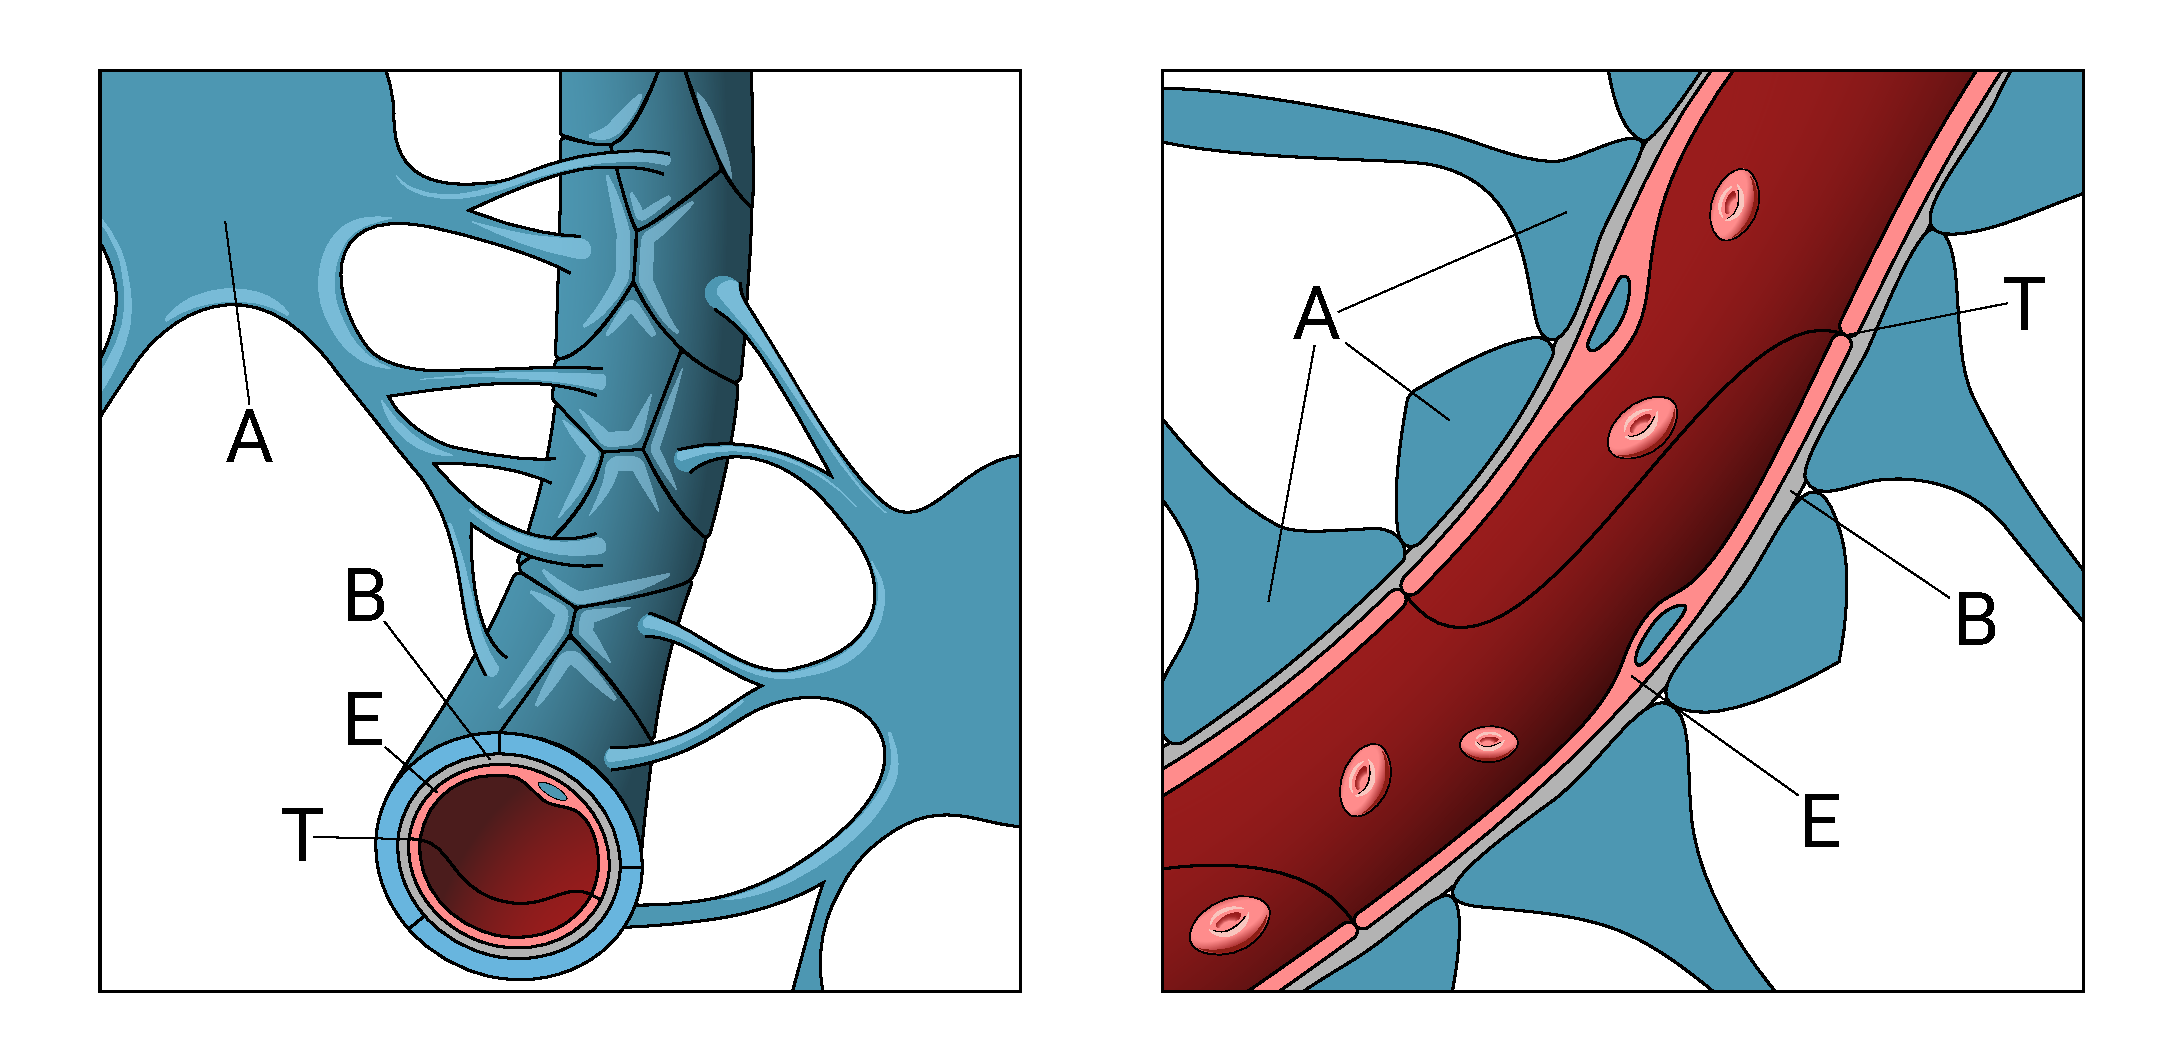
\includegraphics[width=\textwidth]{figures/bbb}
\caption[Schematic Display of the Blood-Brain-Barrier.]{\textbf{Schematic Display of the Blood-Brain-Barrier.} The blood-brain-barrier surrounds virtually every capillary in the CNS. A: Astrocyte, B: Basal Membrane, E: Endothelial Cell, T: Tight Junction. Modified from Lobentanzer \& Klein, 2019.\cite{Lobentanzer2019b}
\label{fig:bbb}}
\end{figure}

Until very recently, studies aiming to clarify the transcriptional profiles of neurons applied either microarray technology or \ac{seq} (also known as deep sequencing or next generation sequencing). For these methods, several cubic millimetres of brain tissue are required at the least; often, cubic centimetres are used. In contrast, the diameter of neuronal somata is usually in the micrometre range. Thus, the resolution of the method and the actual cellular resolution differ by a factor of approximately \num{1000}. Additionally, even among the neuronal population, there is considerable heterogeneity and transcriptomic plurality; single brain regions rarely consist of less than 30 different neuron types, tightly packed next to each other, each with their own transcriptional identity.\cite{Darmanis2015, Zeisel2015, Tasic2016, Habib2016} Newest studies, deciphering the murine nervous system by sequencing of \num{500000} individual cells, show that neuron diversity is very similar regardless of brain region.\cite{Zeisel2018} These circumstances hold true for any mammal, and most of our knowledge stems from the analysis of our favourite research animal, the mouse. In humans, the diversity is only exacerbated; in fact, the elevation in \ac{cns} complexity, which is only made possible by enhanced transcriptional control, may be the reason for our superior cognitive abilities.\cite{}

Cholinergic neurons always constitute a minority in any neuronal population, sometimes to extremes. Most tissues are dominated by few neuron types, such as pyramidal cells in the cortex. The most common neurotransmitter types are GABAergic (inhibitory) and glutamatergic (excitatory), each with several subtypes. It is estimated that more than 80\% of cortical neurons are excitatory, and more than 90\% of synapses release glutamate.\cite{Raichle2002} There are two major cholinergic regions in the mammalian brain: the striatum is fairly well-populated with rather large cholinergic interneurons, and the basal forebrain holds a large amount of (smaller) cholinergic projection neurons (compare Fig.\,\ref{fig:projections}). However, in transcriptomic analyses, these tissues are seldom used, maybe due to lack of scientific interest, or because they are notoriously hard to access (the basal forebrain is small and deeply imbedded in the midbrain). The cortex, particularly the neocortex, is most often the tissue of choice in these studies, due to its scientific interest and accessibility. Though it contains only a miniscule amount of cholinergic interneurons whose transcriptional identity is still a matter of debate, several of the recent single-cell \ac{seq} approaches have independently identified cholinergic interneurons in cortical regions (see Fig.\,\ref{fig:singlecell}).

\section{Cortical Single-Cell RNA Sequencing} \label{sec:cellculture:singlecell}
The impact of transcriptional dynamics on any disease depends on co-expression of the relevant genes in the affected cell. Selection of a model therefore has to take co-expression into account. In particular, if neurokines are to possess any relevance for cholinergic properties of central nervous cells, the cells in question would have to express molecular machinery required to receive neurokine signals. The advent of single-cell \ac{seq} for the first time enables the resolution of gene expression on a cellular basis, and thus the disentangling of spatially close individual neuron types (and other, non-neuronal \ac{cns} cells); most of this information is lost in \ac{seq} performed on brain homogenate, even of a small biopsy. Differences in genes are reduced to the universally expressed »housekeeping« genes, save the most extreme perturbations. In \acp{mir}, this circumstance is only exacerbated, in parallel to their even more tissue-specific expression.

\begin{method}
\subsection{Single-cell Dataset Processing}

To provide a detailed tally of transcriptional subtypes in the \ac{cns}, publicly available single-cell \ac{seq} datasets of suitable tissues were analysed towards their cholinergic properties. All studies that were available at the time focused on some subsection of the cortex (visual or somatosensory) or the hippocampus. The data provided by those studies were in some cases pre-aggregated to represent classes of single neurons with similar transcriptomes (Fig.\,\ref{fig:singlecell}\,A\&B\cite{Zeisel2015, Tasic2016}); in other cases, every single neuron was represented (Fig.\,\ref{fig:singlecell}\,C\&D\cite{Darmanis2015, Habib2016}). 

An important quality-related parameter of a single-cell \ac{seq} experiment is the achieved sequencing depth per single sequenced cell. Some of the screened datasets do not provide sufficient depth to resolve genes with medium expression, which includes our primary cholinergic markers \textit{\ac{chat}} and \textit{\ac{slc}}. The datasets which did provide adequate sequencing depth were filtered for their expression of these markers, and additionally characterised by their expression of common markers for cell types to be expected in the \ac{cns}. Raw data were downloaded from their respective sources and imported into the R environment, where they were converted into similar format. Numeric expression values of each dataset were normalised to \ac{tpm} to allow comparison (with counts $n$ and transcript length $\ell$ of gene $A$ and all genes $i$ per sample): $$TPM_A = \frac{\frac{n_A}{\ell_A}}{\sum_i \frac{n_i}{\ell_i}}\times 10^6$$

For graphical display, TPM were further normalised to a range of \num{0}-\num{1}. The transcripts of interest were filtered from each dataset and plotted as heatmaps. Plotted were only samples that expressed \emph{CHAT}, \emph{SLC18A3} (also known as vAChT), and/or \emph{SLC5A7} (also known as HACU).

\subsection{microRNA and Transcription Factor Targeting Predictions}
Making use of the information aggregated in \emph{miRNeo}, the genes identified as being expressed in cholinergic neurons were subjected to permutation targeting analyses of miRNAs and TFs. Genes were assumed to be expressed in cholinergic neurons if they were expressed in more than one individual sample in all single-cell \ac{seq} datasets (Fig.\,\ref{fig:singlecell}\,A-D). The TFs identified as active towards cholinergic genes in cholinergic neurons were additionally subjected to another round of miRNA targeting permutation analysis. Targeting of genes with random selections of miRNAs and TFs were permuted \num{100000} times to estimate \ac{fdr}. Statistical significance of the miRNA$\to$gene or TF$\to$gene interactions was assumed at FDR < 0.05.

\end{method}

\subsection{Single-cell Expression of Cholinergic and Neurokine Transcripts}

The identified samples provide an overview of potentially cholinergic cells in the sampled brain regions, and allow an assessment of the functional type and gene co-expression patterns in central cholinergic cells (Fig.\,\ref{fig:singlecell}). Most cells identified as cholinergic by this definition expressed the general neuronal marker \textit{\acs{rbf}}, also known by its trivial name NeuN, but not the microglial marker \textit{\acs{aif}}. Few cells (or clusters of cells) expressed non-neuronal markers such as \textit{\acs{gfap}} (astrocytes) or \textit{\acs{oli}} (oligodendrocytes), hinting at sparse non-neuronal cholinergic functions. In agreement with our findings, cells or clusters identified as cholinergic by the authors of the respective studies\cite{Zeisel2015, Tasic2016} (also by personal communication with Peter Lönnerberg) were classified as interneurons and co-expressed a number of known phenotypic neuronal markers, such as \textit{\ac{sst}} and \textit{\ac{vip}}.

The identified cholinergic cells also revealed a constant co-expression with neurokine-related genes, particularly the transmembrane neurokine receptors \ac{lifr} and \ac{ilst}, demonstrating a capacity to receive and process neurokine signals. In contrast, the high affinity receptor for \ac{ngf}, \textit{NTRK1}, is not co-expressed in mature (NeuN-positive) cholinergic neurons in the analysed regions, fundamentally distinguishing these cells from the basal forebrain cholinergic projection neurons.

\begin{figure}[ht]
\centering
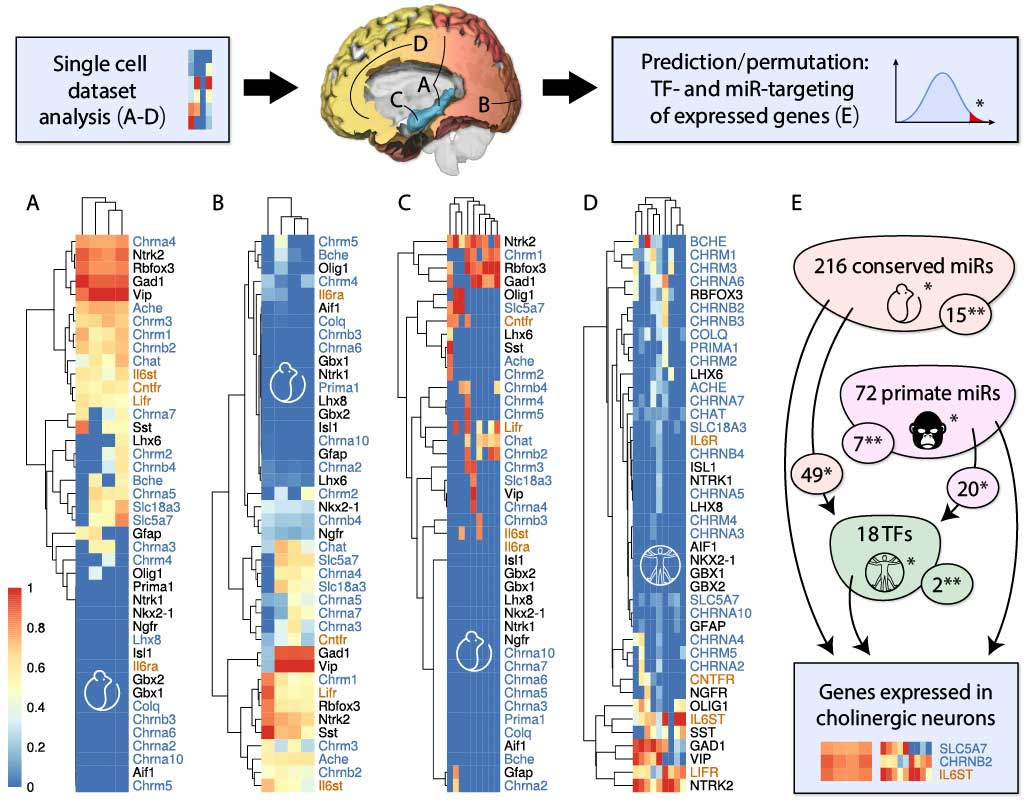
\includegraphics[height=10cm]{figures/singlecell}
\caption[Single-Cell Sequencing of CNS Tissues.]{\textbf{Single-Cell Sequencing of CNS Tissues.} Expression patterns of cholinergic and cholinergic-related genes were analysed using web-available single-cell sequencing datasets. Expression was normalised to reflect a span between 0 and 1. \textbf{A)} Clustered single-cell sequences from transgenic mouse somatosensory cortex and hippocampus.\cite{Zeisel2015} \textbf{B)} Clustered single-cell sequences from transgenic mouse visual cortex.\cite{Tasic2016} \textbf{C)} Single-nucleus sequencing of adult mouse hippocampus.\cite{Habib2016} \textbf{D)} Single-cell sequencing of the human developing neocortex.\cite{Darmanis2015} \textbf{E)} Nested regulatory circuits comprised of evolutionarily conserved and primate-specific miRNAs and transcription factors active towards genes expressed in cholinergic neurons were identified by permutation targeting analysis via \emph{miRNeo}. *: p < 0.05, **: p < 0.001.
\label{fig:singlecell}}
\end{figure}

\subsection{Nested Regulatory Networks of miRNAs and Transcription Factors in Single Cholinergic Cells}
Permutation targeting analyses revealed a nested regulatory interaction between 72 primate-specific miRNAs, 216 conserved miRNAs, and 18 TFs towards cholinergic genes expressed in cholinergic neurons (Fig.\,\ref{fig:singlecell}\,E). TFs targeting cholinergic genes were in turn targeted by 49 conserved and 20 primate-specific miRNAs that also targeted cholinergic genes directly.

\begin{method}

\subsection{Transcript Clustering Based On Expression}

Hierarchic clustering was applied to expression data to identify functional grouping of transcripts and cells based on co-expression. Initially, samples (i.e., single cells, pre-aggregated clusters of cells, or brain regions) are compared using a similarity- or distance-matrix (where similarity = \num{1} - distance). The similarity measure is based on a computation according to the method used. For instance, Euclidean distance between two gene expression vectors (i.e., samples) of length $n$ is the distance between points $p$ and $q$ in $n$-dimensional space, defined by: $$d_E(p, q) = \sqrt{\sum_{i=1}^{n} (p_{i}-q_{i})^2}$$

Applying this measure to all pairwise combinations of samples results in a dissimilarity matrix that can be converted to a hierarchy using one of several clustering algorithms. Generally, samples are grouped by their similarity. Initially, each sample is assigned to its own cluster, and then, cluster number is iteratively reduced by joining the closest clusters. This results in a hierarchic tree of samples, that can be »cut« at any height to yield an arbitrary number of clusters. In biological analyses, the method after Ward (in R, »Ward.D2«) is often used.\cite{Murtagh2014}

Due to the structure of the data (small number of entities compared to whole genome analysis, repetition of zeroes in individual samples), the Bray-Curtis dissimilarity\cite{Bray1957} is superior to Euclidean distance. Bray-Curtis dissimilarity is defined as: $$d_{BC}(p, q) = \frac{2C_{p, q}}{S_p+S_q}$$ Where $C$ is the sum of the lesser expression values common to both vectors $p$ and $q$, and $S$ is the total number of transcripts expressed in each sample (i.e., values greater than zero in each vector). Based on this measure, the samples were clustered according to their cholinergic gene expression levels using Ward's method to yield five separate clusters. Intermediary clustering results (not shown) revealed a uniform distribution of \ac{acly}, yielding no additional information; thus, it was removed. Also removed for the purpose of clustering were the non-neuronal nicotinic receptor subunits $\upalpha$\num{1}, $\upbeta$\num{1}, $\upgamma$, $\updelta$, and $\upepsilon$. 

\end{method}

\subsection{Co-Expression of Functional Groups of Cholinergic Transcripts}
Hierarchic clustering of cholinergic transcripts in each of the datasets revealed a grouping of cholinergic transcripts according to their biological function. Table \ref{tab:chol-clusters} shows considerable uniformity in two single-cell mouse datasets, which diverge substantially from the brain-region- and TF-based human set. Generally, clustering shows separation of at least 3 groups of cells, one of which is the classic \emph{cholinergic} neuron with genes for synthesis and transport of acetylcholine. Due to the frequent co-expression of \emph{\ac{chat}} and \emph{\ac{slc}} in neurons, it is safe to assume the \emph{\ac{slc}} as a viable substitute for \emph{CHAT} expression and clustering in the FANTOM5 data of Marbach \emph{et al.}\cite{Marbach2016} (for more details, see Section \ref{sec:database:tf}). In the single-cell datasets, the \emph{CHAT} gene is expressed in parallel with the two cholinergic transporters, without exemption. The other groups could be described as \emph{receptive} neuron (not cholinergic as the aforementioned, but different types of cholinergic receptors and esterase) and other, rather specialised groups, probably comprising various glial cells. These last, specialised groups are not very visible in the human dataset, which lacks the single cell resolution of the mouse datasets and therefore includes glial cells in every sample of any region. Therefore, differences in cholinergic gene expression patterns derived from Marbach \emph{et al.} are likely the result of the numbers and dominant types of cholinergic neurons in the respective regions.

Functional stratification of cholinergic genes is also visible in a dendrogram of gene clusters from all four analysed single-cell sequencing datasets (Fig.\,\ref{fig:chol-clusters}). While there is variability in the composition of receptor subunits (which is to be expected regarding the different sampled brain regions), the core cholinergic genes (such as \emph{CHAT}, \emph{SLC18A3}, \emph{SLC5A7}, and \emph{ACHE}) associate similarly in all datasets. Notably, the distinction between a \emph{cholinergic} and a \emph{cholinoceptive} neuron is always visible by a grouping of, on one hand the synthesis, vesicular packaging, and reuptake of \ac{ach}, and on the other hand, cholinergic receptors and signal termination by AChE.

\noindent\begin{minipage}{\linewidth} %both fig and table on same page

\sffamily
\small
\centering
\begin{tabular}{c | c | c | c}
cluster & Zeisel et al & Tasic et al & Marbach et al \\
\hline
\hline
I & \makecell{Ache, Chrm1, \\Chrm2, Chrm3, \\Chrm4, Chrna4, \\Chrna5, Chrna7, \\Chrnb2} & \makecell{Ache, Chrm1, \\Chrm2, Chrm3, \\Chrm4, Chrna2, \\Chrna4, Chrna5, \\Chrna7, Chrnb2, \\Chrnb4} & \makecell{CHRM1, CHRM2, \\CHRM5, CHRNA2, \\CHRNA4, CHRNA6, \\CHRNB2, CHRNB3} \\ \hline
Ib&  &  & \makecell{ACHE, BCHE, \\CHRNA3, CHRNB4, \\PRIMA1} \\ \hline
Ic& &  & CHRM3 \\ \hline
Id&  &  & CHRNA5, CHRNA9 \\ \hline
II& \makecell{Chat, Chrnb4, \\Slc18a3, Slc5a7} & \makecell{Chat, Chrm5, \\Chrna3, Slc18a3, \\Slc5a7} & SLC18A3, SLC5A7 \\ \hline
III& \makecell{Chrm5, Chrna10, \\Chrna3} & Chrna10 &  \\ \hline
IV&Bche, Prima1 & Bche, Prima1 &  \\ \hline
V& \makecell{Chrna2, Chrna6, \\Chrnb3} & Chrna6, Chrnb3 &  \\
\end{tabular}
\captionof{table}{\textbf{Cholinergic Transcript Clusters According to Cell Type vs. Brain Region.} The two transgenic mouse datasets from Zeisel \emph{et al.}\cite{Zeisel2015} and Tasic \emph{et al.}\cite{Tasic2016} show high similarity in transcript distribution. With high likeliness, cluster I is a group of postsynaptically cholinergic, »receptive« cells. Cluster II represents the classic \emph{cholinergic} neuron, with synthesis, vesicular packaging and ACh-reuptake genes. The transcription factor-based dataset of Marbach \emph{et al.}\cite{Marbach2016} depends on whole brain regions instead of single cells to determine similarity, and thus yields distinctly different classification. However, it also distinguishes between cholinergic synthesis (with \emph{SLC18A3} as a substitute for \emph{CHAT} expression) and cholinoceptive functions.}
\label{tab:chol-clusters}

\vspace{30pt}

\centering
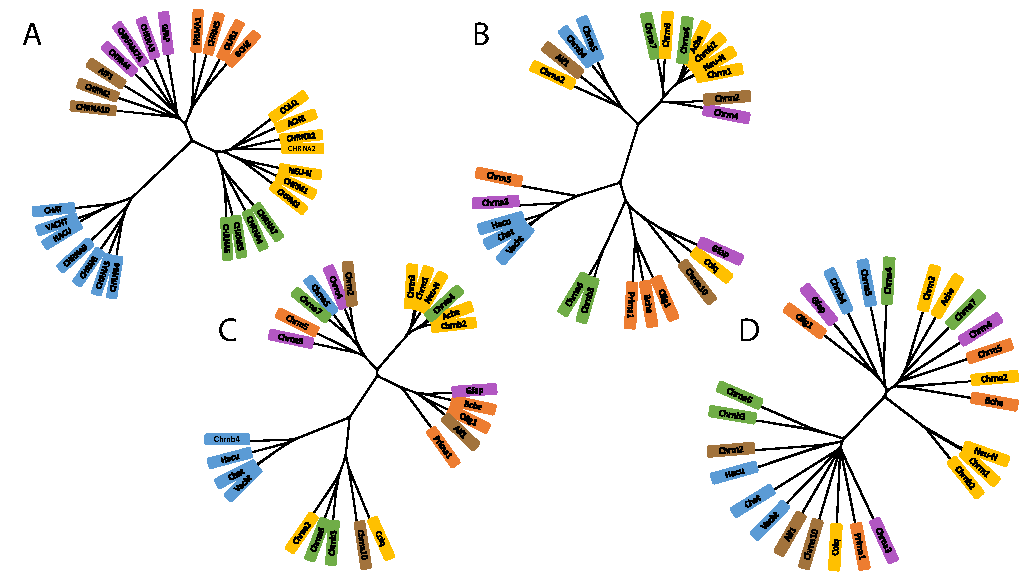
\includegraphics[width=\textwidth]{figures/chol-clusters}
\captionof{figure}[Clusters of Cholinergic Transcripts in Single-Cell Sequencing.]{\textbf{Clusters of Cholinergic Genes in Single-Cell Sequencing.} Cholinergic genes were clustered using Bray-Curtis dissimilarity in four public data sets of single-cell sequencing. The displayed dendrograms visualise the distance between the genes across all samples. Gene clusters were coloured by grouping in Darmanis \emph{et al.}\cite{Darmanis2015} (A). Notably, genes clustered according to their biological function, for instance, CHAT, vAChT and HACU always are closely associated (blue), as are the genes comprising the putative »cholinoceptive« neuron (yellow). \textbf{A)} Single-cell sequencing of the human developing neocortex.\cite{Darmanis2015} \textbf{B)} Clustered single-cell sequences from transgenic mouse visual cortex.\cite{Tasic2016} \textbf{C)} Clustered single-cell sequences from transgenic mouse somatosensory cortex and hippocampus.\cite{Zeisel2015} \textbf{D)} Single-nucleus sequencing of adult mouse hippocampus.\cite{Habib2016} Marker genes are: NeuN - neurons; OLIG1 - oligodendrocytes; AIF1 - microglia; GFAP - astrocytes.
\label{fig:chol-clusters}}

\end{minipage}

\clearpage
